\begin{figure}[H]
    \centering
    \begin{adjustbox}{width=3cm,margin=11cm -12cm}
      
\includegraphics[width=12cm]{src/delay/delay-low.png}%
    \end{adjustbox}
    \begin{adjustbox}{width=10.5cm,center}
      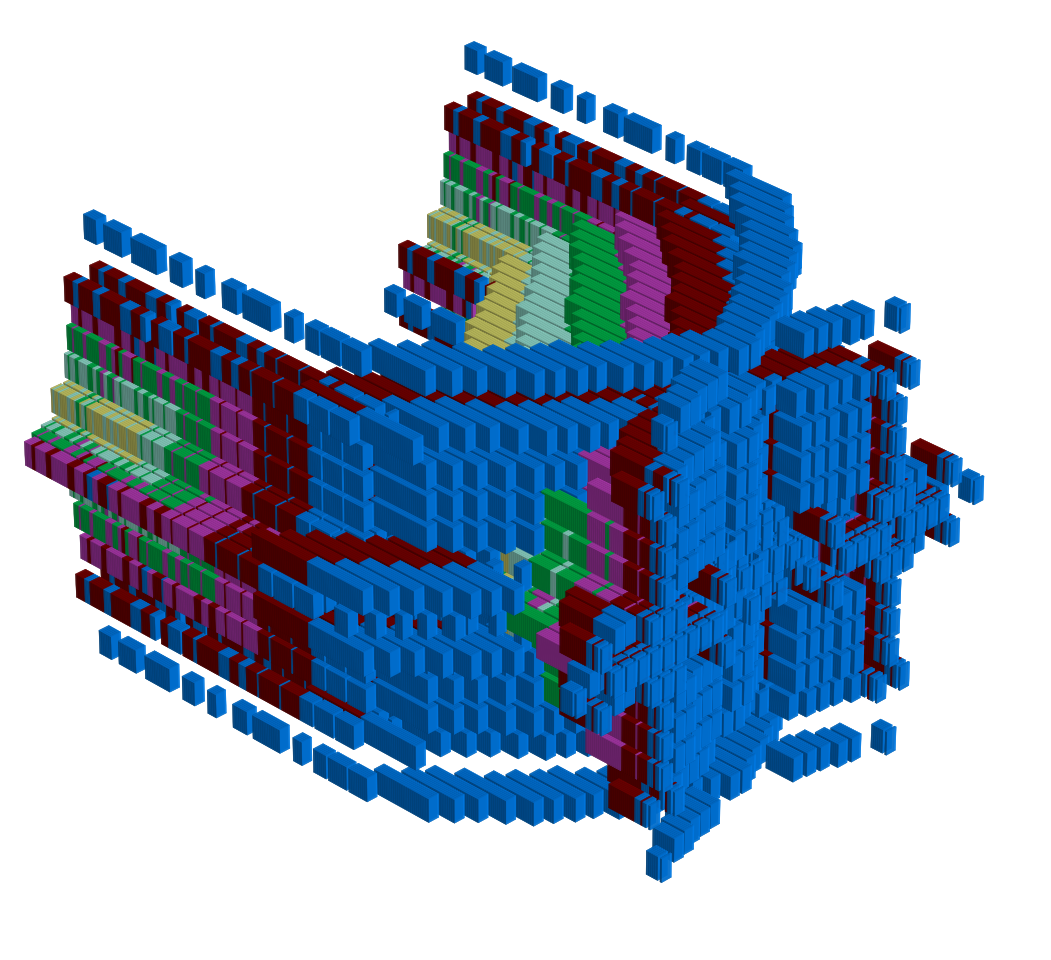
\includegraphics[width=12cm]{src/delay/pattern0-45.png}%
    \end{adjustbox}
    \begin{adjustbox}{width=3cm,margin=11cm -12cm}
      
\includegraphics[width=12cm]{src/delay/delay-high.png}%
    \end{adjustbox}
    \begin{adjustbox}{width=10.5cm,margin=0cm -2cm}
      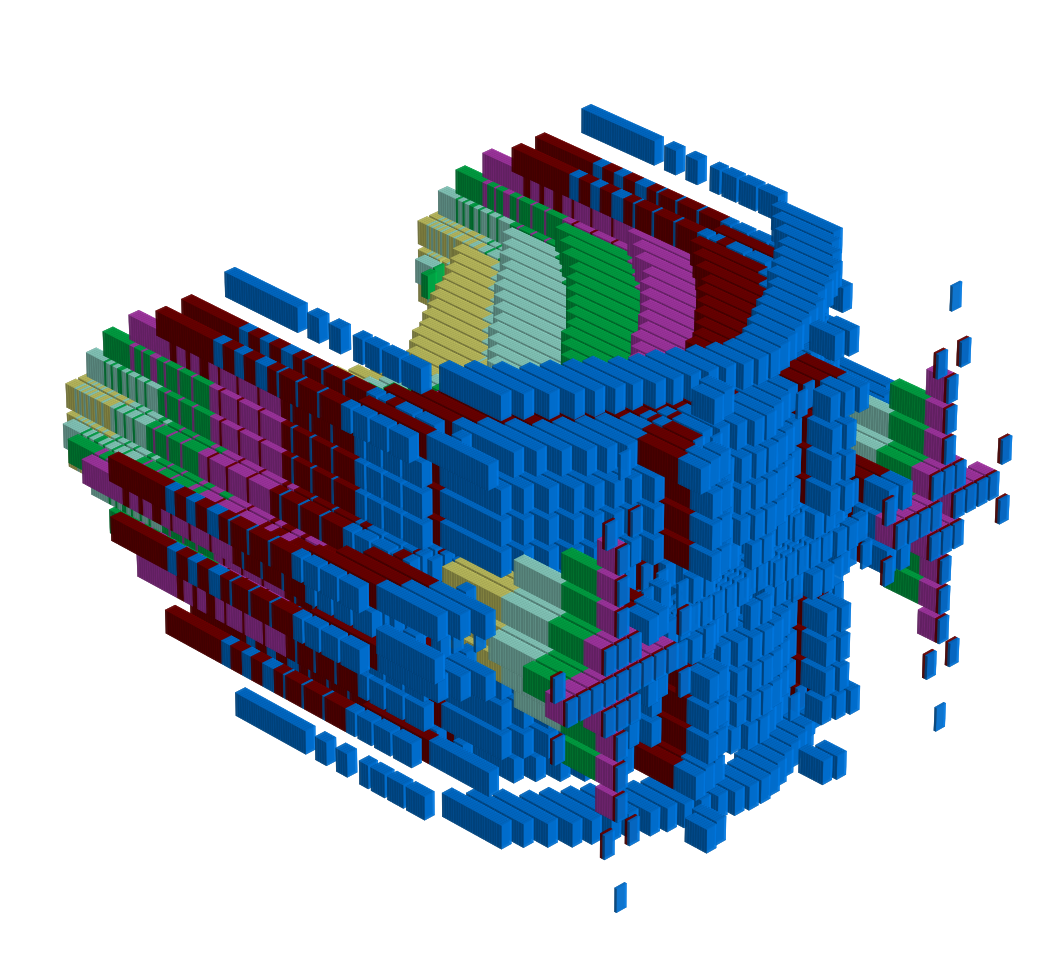
\includegraphics[width=12cm]{src/delay/pattern1-45.png}%
    \end{adjustbox}
    \caption{Effect of low and high values for Smoothing Delay}
\end{figure}
\clearpage

\section*{tentative tracking} 
\label{sec:tracking}
\lstset{style=6502Style}
\lstset{ 
   aboveskip=5pt,
   belowskip=0pt,
}

\begin{definition}[Jeffrey Says]
\setlength{\intextsep}{0pt}%
\setlength{\columnsep}{3pt}%
\begin{wrapfigure}{l}{0.12\textwidth}

\includegraphics[width=\linewidth]{src/callout/psych.png} 
\end{wrapfigure}
\small
\textbf{T to Activate:} Controls whether logic-seeking is used in
the buffer or not. The upshot of this for you is a slightly different
feel - continuous but fragmented when ON, or together-ish bursts
when OFF. Try it.
\end{definition}

\clearpage
\textbf{Lines 1189-1231. \icode{\textbf{CheckKeyboardInput}}} 
\begin{lstlisting}
;-------------------------------------------------------
; CheckKeyboardInput
;-------------------------------------------------------
CheckKeyboardInput   
    ...
MaybeTPressed   
    CMP #KEY_T ; T pressed.
    BNE CheckIfPresetKeysPressed

    ; Toggle tracking on or off.
    LDA trackingActivated
    EOR #$FF
    STA trackingActivated

    ; Use the new setting to get an offset into our screen message.
    ; in txtTrackingOnOff
    AND #$01
    ASL 
    ASL 
    ASL 
    ASL 
    TAY 

    JSR ClearLastLineOfScreen

    ; Display the updated setting of 'tracking'.
    LDX #$00
txtTrackingLoop   
    LDA txtTrackingOnOff,Y
    STA lastLineBufferPtr,X
    INY 
    INX 
    CPX #$10
    BNE txtTrackingLoop

    JMP WriteLastLineBufferToScreen
    RTS 
\end{lstlisting}
\clearpage

\textbf{Lines 1189-1231. \icode{\textbf{MaybeTPressed}}:} 
Pressing \icode{T} toggles tracking on or off. Tracking's on/off state is 
stored in \icode{trackingActivated}, with \icode{\$00} meaning 'off' and
\icode{\$FF} meaning 'on'. This means we can use a neat, economical trick
for toggling the value every time the user presses the 'T' key:

\begin{lstlisting}
    ; Toggle tracking on or off.
    LDA trackingActivated
    EOR #$FF
    STA trackingActivated
\end{lstlisting}

The \icode{EOR} statement performs an exclusive-or that has the neat property of
turning \icode{\$00} into \icode{\$FF} and \icode{\$FF} into \icode{\$00} - equivelent
to switching a value on or off.

This is what the the bit by bit operation looks like when '\icode{EOR \$FF}' turns
\icode{trackingActivated} 'on':

\begin{figure}[H]
  {
    \setlength{\tabcolsep}{3.0pt}
    \setlength\cmidrulewidth{\heavyrulewidth} % Make cmidrule = 
    \begin{adjustbox}{width=7cm,center}

      \begin{tabular}{rllllllll}
        \toprule
        Byte & Bit 7 & Bit 6 & Bit 5 & Bit 4 & Bit 3 & Bit 2 & Bit 1 & Bit 0        \\
        \midrule
        \$00 & 0 & 0 & 0 & 0 & 0 & 0 & 0 & 0 \\
        \$FF & 1 & 1 & 1 & 1 & 1 & 1 & 1 & 1 \\
        \midrule
        Result & 1 & 1 & 1 & 1 & 1 & 1 & 1 & 1 \\
        \addlinespace
        \bottomrule
      \end{tabular}

    \end{adjustbox}

  }\caption*{X-OR'ing \$FF and \$00 gives \$FF, the 'on' value for \icode{trackingActivated}.}
\end{figure}

And this is what it looks like when \icode{EOR \$FF} turns \icode{trackingActivated} 'off' again:
\begin{figure}[H]
  {
    \setlength{\tabcolsep}{3.0pt}
    \setlength\cmidrulewidth{\heavyrulewidth} % Make cmidrule = 
    \begin{adjustbox}{width=7cm,center}

      \begin{tabular}{rllllllll}
        \toprule
        Byte & Bit 7 & Bit 6 & Bit 5 & Bit 4 & Bit 3 & Bit 2 & Bit 1 & Bit 0        \\
        \midrule
        \$FF & 1 & 1 & 1 & 1 & 1 & 1 & 1 & 1 \\
        \$FF & 1 & 1 & 1 & 1 & 1 & 1 & 1 & 1 \\
        \midrule
        Result & 0 & 0 & 0 & 0 & 0 & 0 & 0 & 0 \\
        \addlinespace
        \bottomrule
      \end{tabular}

    \end{adjustbox}

  }\caption*{X-OR'ing \$FF and \$FF gives \$00, the 'off' value for \icode{trackingActivated}.}
\end{figure}
\clearpage

\clearpage
\textbf{Lines 1189-1231. \icode{\textbf{MainInterruptHandler}}} 
\begin{lstlisting}
;-------------------------------------------------------
; MainInterruptHandler
;-------------------------------------------------------
MainInterruptHandler
        ...
        ; Finally, update the pixel buffers with a byte
        ; each for the current pattern.        
UpdatePixelBuffersForPattern    
        INC currentStepCount
        LDA currentStepCount
        CMP bufferLength
        BNE UpdateBaseLevelArray

        LDA #$00
        STA currentStepCount

UpdateBaseLevelArray   
        TAX 
        LDA currentColorIndexArray,X
        CMP #$FF
        BEQ UpdatePositionArrays

CheckIfTrackingActivated
        LDA previousIndexToPixelBuffers
        AND trackingActivated
        BEQ DrawCursorAndReturnFromInterrupt

        TAX 
        LDA currentColorIndexArray,X
        CMP #$FF
        BNE DrawCursorAndReturnFromInterrupt

        STX currentStepCount

UpdatePositionArrays   
        LDA cursorXPosition
        STA pixelXPositionArray,X
        LDA cursorYPosition
        STA pixelYPositionArray,X

        ...
DrawCursorAndReturnFromInterrupt    
        LDA #$01
        STA currentColorToPaint
        JSR PaintCursorAtCurrentPosition
        ; Falls through
\end{lstlisting}
\clearpage

\textbf{Lines 1189-1231. \icode{\textbf{MainInterruptHandler}}:} 
As you may remember the \icode{MainInterruptHandler} runs every 1/60th of a
second.  You may also recall its main job is to fill the pixel buffers (e.g.
pixelXPositionArray, pixelYPositionArray and so on) so that the MainPaintLoop
can use them to paint the screen. 

\textbf{Lines 1189-1231. \icode{\textbf{CheckIfTrackingActivated}}:} 
\icode{trackingActivated} comes into play here. The idea is that if 'tracking'
is enabled then we should do a re-paint of the last entry in the buffers that was
processed by \icode{MainPaintLoop}. Naturally, if a pixel is being painted twice
over this will create a 'tracking' effect, as though the pattern is trailing a 
glowing tail after it.

We use the value in \icode{trackingActivated} to decide whether or not to paint
the previously processed position in the buffers by simply \icode{AND}'ing the
two together.

\begin{lstlisting}
        LDA previousIndexToPixelBuffers
        AND trackingActivated
        BEQ DrawCursorAndReturnFromInterrupt
\end{lstlisting}

If it's zero, we bail out
completely until the next interrupt by jumping to \icode{DrawCursor\-AndReturnFromInterrupt}.
But if we get a non-zero value that means tracking is enabled and 
we should go ahead and refresh the values in the buffers at the index given
by the value in \icode{previousIndex\-ToPixelBuffers}. So we 'fall through' instead to
\icode{UpdatePositionArrays} and a number of other sub-routines that update the
values of the previous position in our pixel buffers.

\clearpage
